% Begin the document and set up the style of the document
\documentclass[a4paper,11pt]{article}

% Install the required packages for the document 
\usepackage{enumitem}
\usepackage{amsmath}
\usepackage{amssymb}
\usepackage{verbatim}
\usepackage{mathtools}
\usepackage{tikz}
\usepackage{nicefrac}
\usepackage{bm}
\usepackage{xlop}

\newcommand{\norm}[1]{\left\lVert#1\right\rVert}


% Page and style settings
%\parskip=8pt
\parindent=0pt
% Right margin
\textwidth=6.25in
% Left margin
\oddsidemargin=0pt
\evensidemargin=0pt
% Bottom margin
\textheight=10in
% Top margin
\topmargin=-0.75in
\baselineskip=11pt
% end of page and other style settings

\renewcommand{\familydefault}{\sfdefault}
\usepackage{calrsfs}
\DeclareMathAlphabet{\pazocal}{OMS}{zplm}{m}{n}

\newcommand{\indep}{\mathrel{\text{\scalebox{1.07}{$\perp\mkern-10mu\perp$}}}}
\newcommand{\p}{\mathbb{P}}
\newcommand{\e}{\mathbb{E}}
\newcommand{\ds}{\displaystyle}
\newcommand{\code}{\texttt}
\newcommand{\HRule}{\rule{\linewidth}{0.5mm}} % Defines a new command for the horizontal lines, change thickness here

\newenvironment{nscentre}
 {\parskip=0pt\par\nopagebreak\centering}
 {\par\noindent\ignorespacesafterend}


\usepackage{fullpage}

\usepackage{titlesec} % Used to customize the \section command
\titleformat{\section}{\bf}{}{0em}{}[\titlerule] % Text formatting of sections
\titlespacing*{\section}{0pt}{3pt}{3pt} % Spacing around sections

\begin{document}
\setlength{\abovedisplayskip}{8pt}{%
\setlength{\belowdisplayskip}{8pt}{%

\begin{nscentre}
	\textbf{COMP9444: Neural Networks and Deep Learning}\\
	\textbf{Assignment 1}\\
\end{nscentre}

\text{Name: Keegan Gyoery}
\hfill
\text{zID: z5197058}

\HRule

\pagenumbering{arabic}
	\section{Part 1: Japanese Character Recognition}
	\begin{enumerate}[leftmargin=*]
		\item NetLin is a fully connected single layer network with 784 input nodes, and 10 output nodes. The data is activated at the output nodes by the \code{log\_softmax} function. Running the command 
			\begin{align*}
				\code{python3 kuzu\_main.py --net lin} 
			\end{align*}
			gives the following confusion matrix,
			\begin{align*}
				\begin{bmatrix}
					770 & 7 & 8 & 3 & 60 & 8 & 5 & 16 & 12 & 7 \\
					6 & 667 & 61 & 37 & 52 & 27 & 23 & 30 & 33 & 50 \\
					8 & 106 & 690 & 59 & 80 & 125 & 145 & 26 & 94 & 92 \\
					14 & 17 & 26 & 760 & 21 & 17 & 9 & 13 & 44 & 4 \\
					31 & 32 & 25 & 16 & 623 & 20 & 25 & 85 & 7 & 54 \\
					63 & 23 & 21 & 55 & 18 & 725 & 25 & 17 & 30 & 32 \\
					2 & 59 & 48 & 12 & 32 & 26 & 721 & 52 & 45 & 19 \\
					61 & 11 & 36 & 18 & 35 & 8 & 21 & 628 & 5 & 28 \\
					28 & 26 & 47 & 28 & 20 & 33 & 10 & 85 & 707 & 38 \\
					17 & 52 & 38 & 12 & 59 & 11 & 16 & 48 & 23 & 676 \\
				\end{bmatrix}
			\end{align*}
			with an accuracy of 6967/10000 or 70\%.
		\item NetFull is a fully connected two layer network with 784 input nodes, and 10 output nodes. With 170 hidden nodes, the model was able to achieve an accuracy of 85\%, the highest accuracy found for different numbers of hidden nodes that were multiples of 10. The data is activated at the hidden nodes by the \code{tanh} function and at the output nodes by the \code{log\_softmax} function. Running the command 
			\begin{align*}
				\code{python3 kuzu\_main.py --net full} 
			\end{align*}
			with 170 hidden nodes gives the following confusion matrix,
			\begin{align*}
				\begin{bmatrix}
					856 & 5 & 8 & 3 & 44 & 8 & 3 & 16 & 11 & 4 \\
					3 & 820 & 10 & 12 & 27 & 11 & 11 & 11 & 27 & 17 \\
					2 & 30 & 826 & 33 & 20 & 69 & 40 & 17 & 24 & 46 \\
					6 & 2 & 46 & 913 & 5 & 11 & 9 & 5 & 39 & 5 \\
					29 & 18 & 13 & 3 & 814 & 15 & 16 & 22 & 6 & 29 \\
					30 & 10 & 22 & 14 & 9 & 834 & 7 & 10 & 10 & 7 \\
					4 & 53 & 24 & 4 & 29 & 26 & 897 & 38 & 28 & 23 \\
					35 & 7 & 12 & 2 & 18 & 3 & 7 & 834 & 3 & 19 \\
					30 & 24 & 22 & 7 & 20 & 17 & 2 & 25 & 844 & 9 \\
					5 & 31 & 17 & 9 & 14 & 6 & 8 & 22 & 8 & 841 \\
				\end{bmatrix}
			\end{align*}
			with an accuracy of 8479/10000 or 85\%.
		\item NetConv is a convolutional network with 2 convolutional layers with max pooling, and a final fully connected layer before the output nodes. The first convolutional layer uses a kernel of size 5, steppping from 1 to 100 nodes. The data is then max pooled using a 2x2 square. The second convolutional layer again uses a kernel of size 5, stepping from 100 to 200 nodes. The data is again max pooled using a 2x2 square. The final fully connected layer steps from 3200 nodes to 10 output nodes. With this architecture and these parameters, the model was able to consistently achieve an accuracy of 93\%. The data is activated in the convolutional layers by the \code{relu} function and at the output nodes by the \code{log\_softmax} function. Running the command 
			\begin{align*}
				\code{python3 kuzu\_main.py --net conv} 
			\end{align*}
			with the above parameters gives the following confusion matrix,
			\begin{align*}
				\begin{bmatrix}
					945 & 3 & 9 & 1 & 17 & 2 & 3 & 6 & 7 & 5 \\
					3 & 933 & 11 & 4 & 5 & 14 & 6 & 5 & 14 & 10 \\
					2 & 7 & 864 & 15 & 2 & 35 & 16 & 4 & 8 & 0 \\
					1 & 1 & 36 & 947 & 4 & 4 & 3 & 1 & 1 & 2 \\
					32 & 11 & 17 & 7 & 928 & 5 & 6 & 6 & 5 & 5 \\
					1 & 1 & 5 & 3 & 3 & 901 & 1 & 1 & 2 & 0 \\
					1 & 29 & 24 & 10 & 13 & 21 & 960 & 10 & 6 & 0 \\
					11 & 6 & 21 & 6 & 14 & 12 & 5 & 946 & 2 & 4 \\
					2 & 3 & 6 & 3 & 8 & 3 & 0 & 3 & 954 & 3 \\
					2 & 6 & 7 & 4 & 6 & 3 & 0 & 18 & 1 & 971 \\
				\end{bmatrix}
			\end{align*}
			with an accuracy of 9349/10000 or 93\%. Using a learning rate of 0.02 gives an accuracy of 95\%.
		\item
			\begin{enumerate}
				\item At a high level view, it's clear that the more complex the model became in these three relatively simple models, that the accuracy increased significantly. That is to say, as we both increased the number of hidden nodes used, and the complexity of the architecture, from simple linear networks to convolutional networks that are pooled, our accuracy increased from 70\% to 93\%. Another point to add is for simple two layer networks, the choice of number of hidden nodes is important, as an incorrect or poor choice can lead to less accuracy than a one layer linear network. That was an important factor to note, that the increase in accuracy with the increase in complexity of the architecture was heavily reliant on choosing the appropriate parameters for the model.
				\item Examining the confusion matrix for the first model, NetLin, its accuracy of 70\% meant a lot of characters were misclassified, however the most common mistakes were classifying the character "ma" as "su", "ha" as "su" and "ki" as "su". Overall, this model struggled to classify "na" and "ya", only achieving about 63\% accuracy in these characters due to their complexity and similarity in sub features to other characters. As "su" is has certain components of the character, in particular the loop, that it shares with the other characters "ha" and "ma", coupled with a lack of hidden nodes to aid in breaking up the amount of work each node must do, these large identifying components of the image give a strong probability of classification as either of the three characters, with the variation in handwriting too large for the small differences the network outputs in terms of their probabilities.
					\bigbreak
					Examining the confusion matrix for NetFull, it is a large improvement over NetLin with only one layer of hidden nodes, attaining an accuracy of 85\% with 170 hidden nodes. The most common misclassifications were "ha" as "su", "wo" as "su" and "su" as "tsu". Overall, NetFull struggles the most in classifying "na", one of the most complex characters in the set. Again, as with NetLin, the reasoning for "su" being the character that NetFull mistakenly thought was correct would be very similar to the reasoning for NetLin, however the relative prominence of the error "wo" as "su" is clear due to the similarity of the two, especially if "wo" is written with poor handwriting.
					\bigbreak
					Examining the confusion matrix for NetConv, it is again another significant improvement, with an accuracy of 93\% with a convolutional architecture, using max pooling. Again, NetConv struggled with "su", misclassifying "ha" as "su" relatively more, as well as "o" as "na", both very understandable due to key features of the characters that are identical, and poor handwriting leading to easy confusion, even for humans. Again, "su" was mistakenly classified the most, achieving only 86\% accuracy for "su", due to the loop feature being similar to features of other characters.
				\item No other architectures were experimented with in my code, however it was interesting to note the impact of an increased learning rate, that allowed for higher accuracies and speeds of success for small increases from the default value of 0.01, in NetConv.
			\end{enumerate}
	\end{enumerate}
	\bigbreak
	\section{Part 2: Twin Spirals Task}
	\begin{enumerate}[leftmargin=*]
		\item See the function code.
		\item PolarNet is a fully connected network with 2 input nodes, and 1 output node. Varying the number of hidden nodes connecting the two layers, the minimum number of nodes to consistently achieve 100\% accuracy within 20000 epochs is 7. The data is activated in the first layer by the \code{tanh} function, and at the output node by the \code{sigmoid} function. Running the command
			\begin{align*}
				\code{python3 spiral\_main.py --net polar --hid 7 --epochs 20000}
			\end{align*}
			gives the following plot for \code{polar\_out.png},
			\begin{figure}[!ht]
				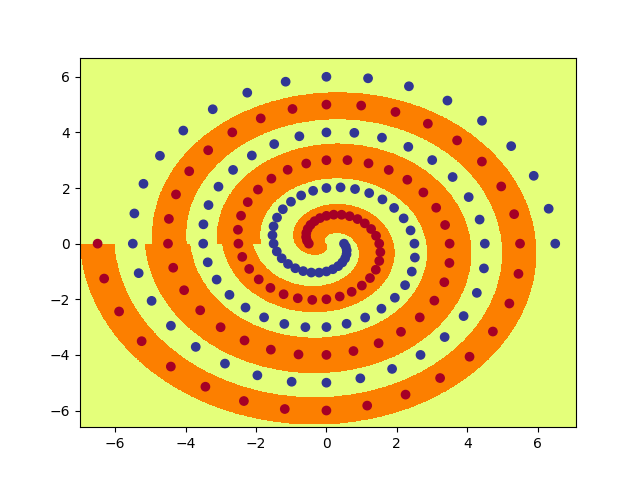
\includegraphics[width=\linewidth]{polarout.png}
			\end{figure}

		\item See the function code.
		\item RawNet is a fully connected 3 layer network with 2 input nodes, and 1 output node. Keeping the number of hidden nodes at each of the two hidden layers constant at 15, but varying the initial weights at each layer, the initial weight of 0.25 consistently achieved an accuracy of 100\% in 20000 epochs. The data is activated in the first and second layers by the \code{tanh} function, and at the output node by the \code{sigmoid} function. Running the command
			\begin{align*}
				\code{python3 spiral\_main.py --net raw --init 0.25 --hid 15 --epochs 20000}
			\end{align*}
			gives the following plot for \code{raw\_out.png},
			\begin{figure}[!ht]
				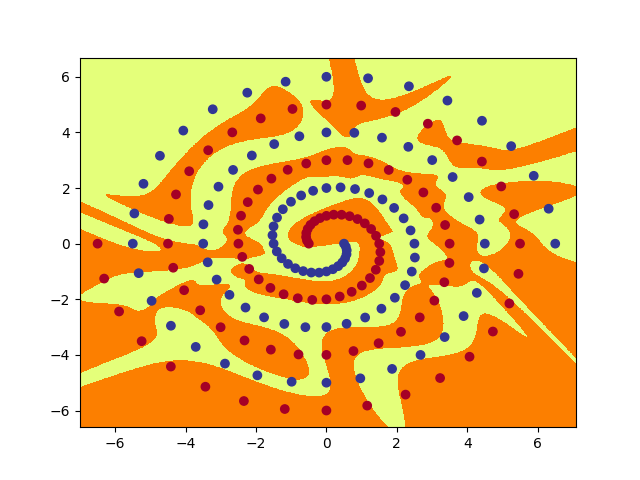
\includegraphics[width=\linewidth]{rawout.png}
			\end{figure}

		\item See the function code.
		\item ShortNet is a fully connected short-cut 3 layer network with 2 input nodes, and 1 output node. Using an initial weight of 0.25 and a learning rate of 0.03 the minimum number of hidden nodes to consistently achieve an accuracy of 100\% in 20000 epochs is 9. The data is activated in all layers except the output layer by the \code{tanh} function, and at the output node by the \code{sigmoid} function. Running the command
			\begin{align*}
				\code{python3 spiral\_main.py --net short --init 0.25 --lr 0.03 --hid 9 --epochs 20000}
			\end{align*}
			gives the following plot for \code{short\_out.png},
			\begin{figure}[!ht]
				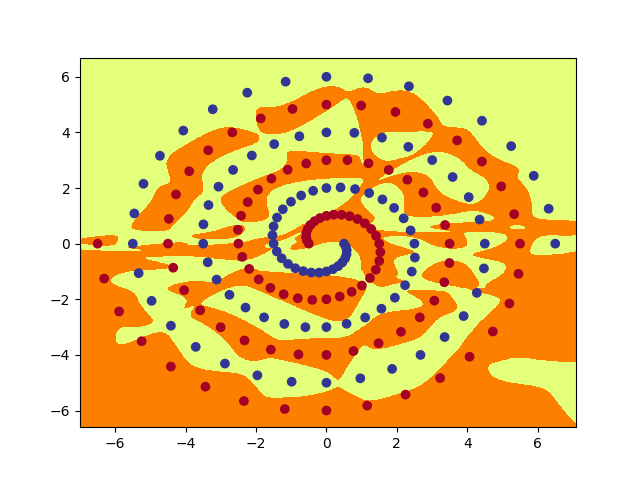
\includegraphics[width=\linewidth]{shortout.png}
			\end{figure}

			\break

		\item I was unable to understand how to plot these values from the hidden node onto the graph at all. I was able to get the activation for each node with the command \code{output = net.h1[:,node]}, however I did not understand how to plot these values once they had been run through the \code{pred = (output >= 0.5).float()} line. The graph was plotted on a specific size grid that was fed through the network to determine the overall activation at each point on the graph, however I was unsure how to feed the grid through the tensor that resulted from a particular node's activation. I understand that this is what I was required to do, I simply had no idea how to implement this in the code, and as a result I have no graphs for each node to include in my report. If you run the code in the function, it will provide the activation values, but will not graph them correctly at all.
		\item Starting with PolarNet, the output function is clearly a spiral, due to the conversion of input into polar coordinates, allowing the neural network to classify using polar coordinates which is far superior for mapping circular objects in the cartesian plane. For RawNet, the output function has contiguous sections that rarely will cross the blue spiral, and only do some in some places. The inner areas of the spiral strongly mimic the results computed from PolarNet, as well as having large areas activated below the spirals as well. RawNet gave areas of activation that were largely contiguous and almost all areas were joined together. In the case of ShortNet, the areas of activation were more fractured relative to RawNet, however, had far better linkage between the various areas provided by the output function, and only had activated areas that were outside of the spiral in the bottom hemisphere of the spiral. Each of RawNet and ShortNet seek to separate each point into a partition of the spiral that contains none of the incorrect points, doing so by creating functions for each node that isolate a set of the points, and in conjunction, each node works together to form a full picture of isolated sections of the spiral.
			\bigbreak
			Both the functions for RawNet and ShortNet are quite seemingly unstructured and more random on a macro scale, but with linkages between the small substructures of the output function. These two functions seem more natural and likely to be representative of a brain pattern or thought process, linking smaller features together to form a complete idea that seems on a macro scale random. The output function for Polar Net is very structured and thus much less likely to be naturally occuring, and seemingly more man made or influenced. However, structure is necessary in representation for deep learning tasks, as otherwise classification is extremely difficult, as is understanding input. 
			\bigbreak
			For both RawNet and ShortNet, initial values for the weights were significantly important, especially for smaller number of nodes, as there was a very tight set of ranges that would alllow the network to achieve 100\% accuracy. As the number of nodes is increased, the range of initial weight values that will lead to a solution grows. Similar with learning rate, RawNet required a very small learning rate, as anything over 0.05 led to significant see-sawing of accuracy, despite fast intial growth in accuracy, it introduced severe fluctuations that decreased the possibility of 100\% accuracy within 20000 epochs. ShortNet was more tolerant of initial weight values and learning rate, and was less susceptible to see-sawing or large fluctuations with an increase in learning rate, although again, there came a point where learning was no longer progressing. A small increase in the learning rate for ShortNet produced a noticeable increase in the rate of success.
	\end{enumerate}
\end{document}
